\documentclass[8pt,a5paper]{extarticle}
\usepackage[margin=1cm]{geometry}
\usepackage[utf8]{inputenc}
\usepackage[IL2]{fontenc}
\usepackage[czech]{babel}
\usepackage{microtype}
\usepackage{amssymb}
\usepackage{amsthm}
\usepackage{amsmath}
\usepackage{xcolor}
\usepackage{graphicx}
\usepackage{wasysym}
\usepackage{multicol}

\usepackage[inline]{enumitem}

\newcommand{\R}{\mathbb{R}}

\newcommand{\hint}[1]{{\color{gray}\footnotesize\noindent(Nápověda: #1)}}

% \DeclareMathOperator{\tg}{tg}
% \DeclareMathOperator{\cotg}{cotg}
% \DeclareMathOperator{\arctg}{arctg}

\setlist[enumerate]{label={(\alph*)},topsep=\smallskipamount,itemsep=\smallskipamount,parsep=0pt,itemjoin={\quad}}
\setlist[itemize]{topsep=\smallskipamount,noitemsep}

\def\tisk{%
\newbox\shipouthackbox
\pdfpagewidth=2\pdfpagewidth
\let\oldshipout=\shipout
\def\shipout{\afterassignment\zdvojtmp \setbox\shipouthackbox=}%
\def\zdvojtmp{\aftergroup\zdvoj}%
\def\zdvoj{%
    \oldshipout\vbox{\hbox{%
        \copy\shipouthackbox
        \hskip\dimexpr .5\pdfpagewidth-\wd\shipouthackbox\relax
        \box\shipouthackbox
    }}%
}}%

\let\results\newpage
\let\endresults\relax

\def\resultssame{%
    \long\def\results##1\endresults{%
        \vfill
        \noindent\rotatebox{180}{\vbox{##1}}%
    }%
}


\newtheorem*{poz}{Pozorování}

\theoremstyle{definition}
\newtheorem{uloha}{\atr Úloha}
\newtheorem*{bonus}{Bonus}
\newtheorem*{defn}{Definice}

\pagestyle{empty}

\let\ee\expandafter

\def\vysld{}
\let\printvysl\relax

\makeatletter
\long\def\vyslplain#1{\ee\ee\ee\gdef\ee\ee\ee\vysld\ee\ee\ee{\ee\vysld\ee\printvysl\ee{\the\c@uloha}{#1}}}
\def\vyslalph#1{\edef\tmpuloha{{\the\c@uloha}{\alph{enumi}}}\ee\ee\ee\gdef\ee\ee\ee\vysld\ee\ee\ee{\ee\vysld\ee\printalphvysl\tmpuloha{#1}}}
\let\vysl\vyslplain

\def\locvysl#1{\ee\gdef\ee\locvysld\ee{\locvysld\item #1}}
\let\lv\locvysl

\newenvironment{ulohav}[1][]{\begin{uloha}[#1]\gdef\locvysld{\begin{enumerate*}}}{\ee\vyslplain\ee{\locvysld\end{enumerate*}}\end{uloha}}
\def\stitem{\@noitemargtrue\@item[$\star$ \@itemlabel]}

\makeatother

\def\atr{}
\def\basic{\def\atr{\llap{\mdseries$\sun$ }\gdef\atr{}}}
\def\interest{\def\atr{\llap{$\star$ }\gdef\atr{}}}
\def\iinterest{\def\atr{\llap{$\star\star$ }\gdef\atr{}}}
\let\mb\mathbf


\begin{document}

% \tisk
% \resultssame

\section*{24. Rozloučení s analytickou geometrií}


\begin{uloha}\label{tecna-parabola}
Mějme parabolu $r$ danou rovnicí $-2(x+1)=(y-1)^2$.
Nalezněte tečny k $r$ z bodu $B[3;2]$. \vysl{$x-2y+1=0$ v bodě $[-3;-1]$ a $x+4y-11=0$ v bodě $[-9;5]$}
\end{uloha}

\begin{uloha}
Stejné $r$ a $B$ jako v Úloze \ref{tecna-parabola}, ale nyní se mají najít všechny přímky procházející $B$, které mají s $r$ právě jeden společný bod.\vysl{kromě těch dvou tečen to je ještě $y=2$}
\end{uloha}

\begin{uloha}
Kružnice $k$ má střed v počátku a poloměr $1$. Parabola $r$ má za osu souměrnosti osu $x$, její ohnisko je \uv{vpravo} od vrcholu a její parametr je $\frac12$; určete souřadnice jejího vrcholu tak, aby měla s $k$ společné právě dva body.\vysl{$\bigl[-\frac54; 0\bigr]$ a pak všechny $[s;0]$, kde $s \in (-1;1)$}
\end{uloha}

\begin{ulohav}
V závislosti na parametru $t \in \R$ rozhodněte, o jaký geometrický útvar se jedná:
\begin{enumerate*}
    \item $x^2 + y^2 = t$,\lv{$t>0$: kružnice, $t=0$: bod, $t<0$: prázdná množina}
    \item $x^2 + ty^2 = 1$,\lv{$t<0$: hyperbola, $t=0$: dvě rovnoběžné přímky, $t>0$: elipsa (pro $t=1$ kružnice)}
    \item $x^2 + tx + y^2 = 1$,\lv{vždy jde o kružnici}
    \item $x^2 - y^2 - ty = 1$.\lv{$t\in \{-2;2\}$: dvě různoběžné přímky, $t \notin \{-2;2\}$: hyperbola}
\end{enumerate*}
\end{ulohav}

\begin{uloha}
Určete obecnou rovnici roviny, která prochází body $[3;0;0]$, $[0;2;0]$ a $[0;0;4]$. Napadne vás rychlá metoda, jak to určovat, pokud máte zadány body ležící na osách?\vysl{$\frac13x + \frac12y + \frac14z - 1 = 0$, z čehož je ta metoda snad vidět}
\end{uloha}

\begin{uloha}
Vypočítejte vzdálenost bodu $M[3;-1;4]$ od přímky $AB$, kde $A[0;2;1]$, $B[1;3;0]$.\vysl{$2\sqrt6$} %sb 4.90
\end{uloha}

\begin{uloha}
Najděte obecnou rovnici roviny, která prochází bodem $A[1;-2;4]$ a je kolmá na roviny $\varrho\colon 2x+y-3z+7=0$, $\sigma\colon x-2y-z+4=0$.\vysl{$x+y+2z-2=0$} %sb 4.80a
\end{uloha}

\begin{uloha}
Ukažte na příkladu, že vektorový součin není asociativní, tj. nalezněte tři vektory $\mb u$, $\mb v$, $\mb w$, které budou splňovat $(\mb u \times \mb v) \times \mb w \neq \mb u \times (\mb v \times \mb w)$.\vysl{např. $\mb u=\mb v=\mb e_1$, $\mb w = \mb e_2$}
\end{uloha}

\begin{uloha}
Dokažte, že vzdálenost dvou (nezbytně rovnoběžných) přímek v rovině, jejichž obecné rovnice jsou $p\colon ax + by + c_1 = 0$ a $q\colon ax + by + c_2 = 0$, je dána vztahem
\[ \frac{|c_1-c_2|}{\sqrt{a^2 + b^2}}. \]
\vysl{vzdálenost $p$ a $q$ lze spočítat jako vzdálenost libovolného bodu $q$ od $p$; vezmeme-li libovolný bod $B[x_0;y_0]$ ležící na $q$, pak jeho vzdálenost od $p$ je dána vztahem $\frac{1}{\sqrt{a^2 + b^2}}|ax_0 + by_0 + c_1|$, ovšem $ax_0 + by_0 = -c_2$, protože $B \in q$}
\end{uloha}

\interest
\begin{uloha}
Rovnice $x^2-x-2 x y+y^2-y = 0$ popisuje určitou parabolu. Zkuste odhadnout, jak vypadá, a určit její parametr. \hint{Všimněte si určité symetrie.}\vysl{jde o parabolu s vrcholem v počátku, která je symetrická podle osy $y=x$, parametr je $\frac{\sqrt2}{4}$}
\end{uloha}

\interest
\begin{uloha}
Spočtěte objem toru, jehož \uv{roura} má poloměr 1 a poloměr prázdné části je rovněž 1. \hint{Jde o \uv{rozdíl} dvou rotačních těles.}\vysl{$4\pi^2$}
\[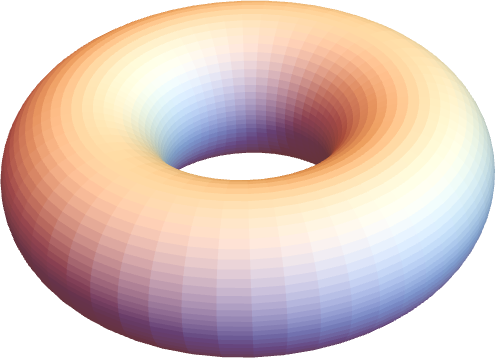
\includegraphics[width=3cm]{torus.png}\]
\end{uloha}


\baselineskip=1.25\baselineskip
\setlist[enumerate]{label=\textbf{(\alph*)},itemjoin={\quad}}

\results
\parindent=0pt
\rightskip=0pt plus1fil\relax
\def\printvysl#1#2{\textbf{#1.} #2\par}
\def\printalphvysl#1#2#3{\textbf{#1}(#2)\ #3\par}
\vysld
\endresults


\end{document}